\chapter{Diage Modelling Language}
In this chapter I will cover the Diage Modelling Language (DML) that is used to visualize the flow of information, some are static and others will wait for the interaction of the player to release this information and ensuring plot progression. \diage uses the symbols to represent the \diage entities as seen in figure~\ref{fig:DMLSymbols}. 
\begin{figure}[h]
	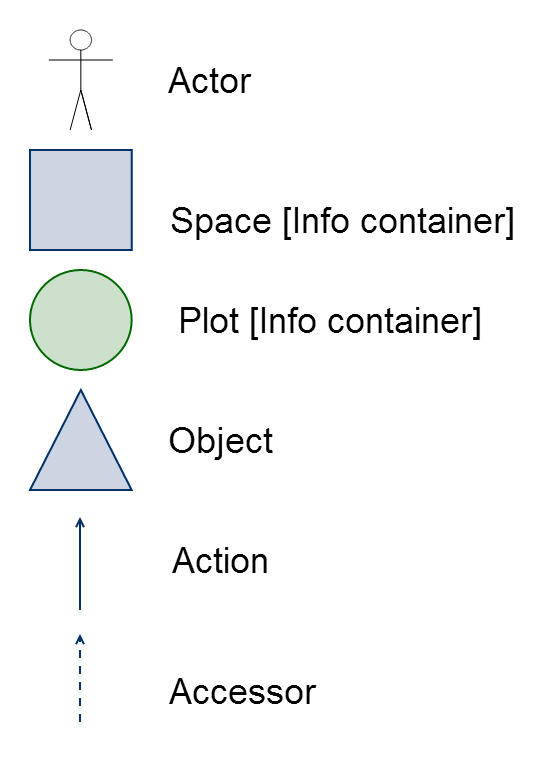
\includegraphics[scale=.3]{symbols}
	\caption{DML Symbols}
	\label{fig:DMLSymbols}	
\end{figure}
\section{Entities}
\diage entities come in four forms; \code{Actors}, \code{Objects}, \code{Spaces} and \code{Events}. The latter two are also information containers which I will discuss in section~\ref{sec:informationcontainers}. The following section will only cover the pure entities; the objects and actors. In conjunction with \code{actions} and \code{accessors} these entities convey story information and plot progression. 
\subsection{Objects}
\diage objects form the basis of all entities. They represent the props and items that we find in the world that have narrative importance. For example; if the Player walks in to a shop \diage does not specify all items that one could buy in the shop, but only those that have plot importance. In terms, these objects should adhere to the \textit{Checkhov's Gun} principle. This dramatic principle states that all objects used in a narrative should eventually be used. I quote: "\textit{One must never place a loaded rifle on the stage if it isn't going to go off. It's wrong to make promises you don't mean to keep.\footnote{\url{http://berlin.wolf.ox.ac.uk/lists/quotations/quotations_by_ib.html}}}"
Objects have three properties; a \code{name}, a \code{ID} and a \code{type} The ID is a unique identifier dependant on the type. And the type is used with actions/accessors as seen in figure~\ref{fig:actions} (Futher discussed in section~\ref{sec:actors}). The name is the noun given to an object within the story context. For example; The player receives the \textit{Skeleton Key of Awesomeness}, but the type is just \code{key} giving it no special properties than any other key. It might make sense to name an object something else than it's type, but a name is not given it defaults to it's type. 
Objects form the world, and all other entities derive from the \diage object. This means that all entities have the same properties as the object, but can extend upon it.
\subsection{Actors}
\label{sec:actors}
An actor is the representation of any one object that can, as the noun implies, act. Examples are the store-clerk, a wandering adventurer or the player. The actor is the only entity that can physically interact with the world, and by doing so the only that can change the world's state. By being able to change the world, the actors are the only entities that can ensure plot progression. 
Just like the object, an actor has three properties; a \code{name}, a \code{ID} and a \code{type}. The type property is used in predefined actions as seen in figure~\ref{fig:actions:npc}. This figure defines that the \code{Player} can \textbf{speak} to all actors of type \code{NPC}. A further glance at figure~\ref{fig:actions} shows some more actions that could be defined for the player actor. These predefined actions tell us that the player can trigger all events and enter all spaces. I will expand upon these actions in section~\ref{sec:actions_and_accessors}.

\section{Information Containers}
\label{sec:informationcontainers}
Information containers are entities that hold story information. A space holds information about it's spacial children, and events release information into spaces when they are resolved. Information containers have the unique property that they are nestable. For example; a space that represents a city can hold several spaces that represents housing. 

\subsection{Spaces}
A space is the representation of any segment of the world or the world itself. As spaces are info containers they are nestable, as mentioned before, but they differ in the fact that they can hold every entity as a child. These children make up the spacial awareness of the space and tells us what information it can pas on to actors. Usually an actor gains all the information a space can give upon the moment it enters the space; when the actor becomes a child object to the space. This can be modified, and some parts of information maybe withheld from the actor, but this is where the events come in.

\subsection{Events}
A event is the odd one out as an entity, as it is the only one that does not represent something within the narrative. A event is the abstraction of information that is released into the story when an actor - usually the player - interacts with it, thus events are used for story pacing and narrative convenience. When we need the state of a space to change we use a event to initiate that change. This only applies on the narrative context of the world, because \diage does not specify everything that happens with in the interactive context. For example; if the player went to a store to buy some cheese to eat. \diage only specifies the store's loss of the cheese, if said food item is a special narrative item. Like a poisonous piece of cheese that the villain left there as a cunning trap for our hero. Events make the world go round and are the dynamic forces in \diage.

\section{Actions and Accessors}
\label{sec:actions_and_accessors}
Actions and accessors are the abstract connectors in \diage. They convey what actors can do (actions) and what knowledge they possess (accessors). Some accessors are implied, due to the fact that an actor might be the child of a space, in other cases these connections are explicitly added to a \diage model. If we review the diagram in figure~\ref{fig:examplediagram} we see that the mayor has no connections whatsoever. This would imply that the Mayor has no knowledge about what's or who's in the store. If we compare that figure to figure~\ref{fig:example:accessors}, we see that the Mayor now has a connection to the Shop, thus we can be sure that the Mayor has the knowledge it would have, if it had been in the shop space itself.

\begin{figure}[ht]
	\centering
	\begin{subfigure}[b]{0.3\textwidth}
		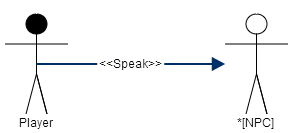
\includegraphics[width=\textwidth]{npc_action}
		\caption{A standard action for NPC interaction}\label{fig:actions:npc}
	\end{subfigure}
	\begin{subfigure}[b]{0.3\textwidth}
		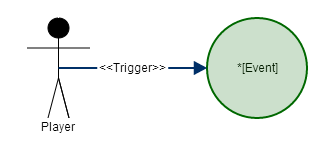
\includegraphics[width=\textwidth]{event_action}
		\caption{A standard action for event interaction}\label{fig:actions:event}
	\end{subfigure}
	\begin{subfigure}[b]{0.3\textwidth}
		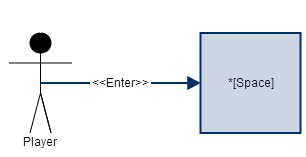
\includegraphics[width=\textwidth]{space_action}
		\caption{A standard action for space interaction}\label{fig:actions:space}
	\end{subfigure}
	\caption{Predefined actions}\label{fig:actions}
\end{figure}

\begin{figure}[ht]
	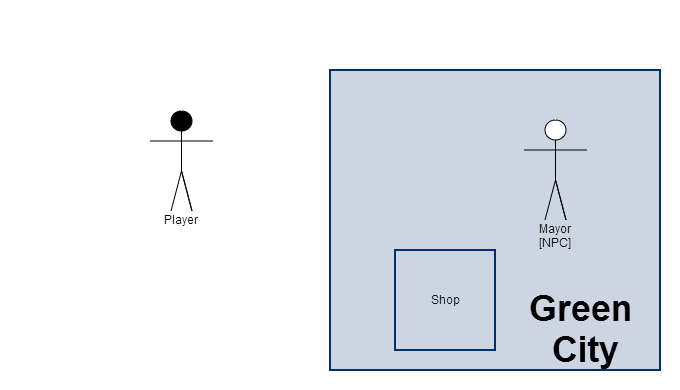
\includegraphics[scale=.5]{diagram_actor_example}
	\caption{An example of a Diage diagram using predefined actions}\label{fig:examplediagram}
\end{figure}
\begin{figure}
	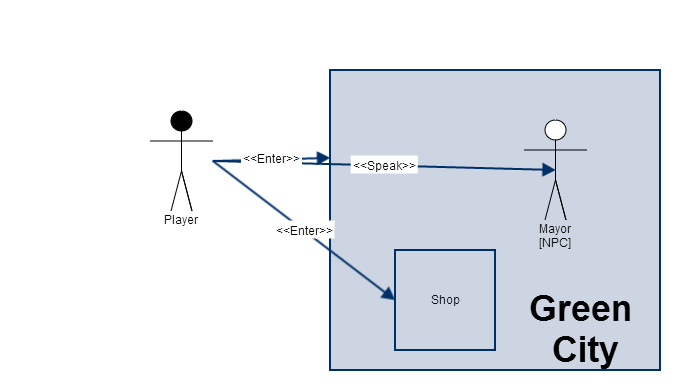
\includegraphics[scale=.5]{diagram_actor_example_verbose}
	\caption{An example of a Diage diagram without using predefined actions}\label{fig:examplediagramverbose}
\end{figure}
\begin{figure}
	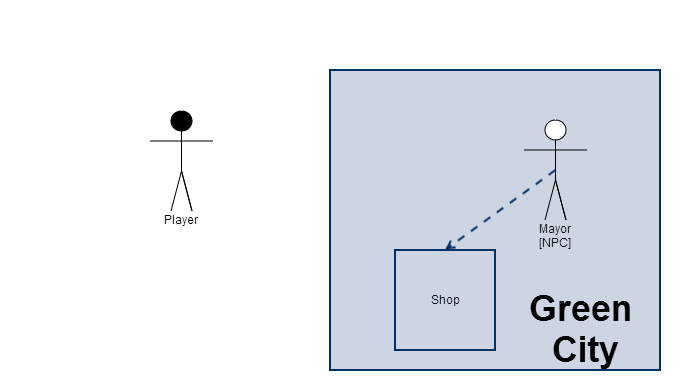
\includegraphics[scale=.5]{diagram_accessor_example}
	\caption{A \diage diagram showing a explicit connection between the Mayor and the Shop}
	\label{fig:example:accessors}
\end{figure}
\section{Diage as a graph}
Diage can be defined by DML, but also as a graph. This form of representation allows us to use graph theory to manipulate and transform the diagram, which we'll cover in the next chapter\footnote{SHOULD BE LEFT FOR FINAL!}

\begin{figure}
	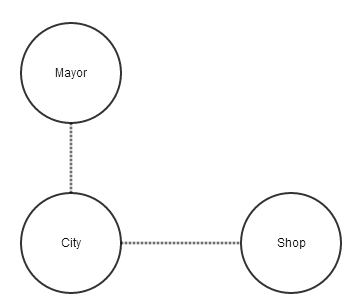
\includegraphics[scale=.5]{diagram_graph}
	\caption{Figure~\ref{fig:examplediagram} as a graph}\label{fig:example:graph}
\end{figure}